% Figure contract
% Core conclusion: the planned stage learns only the body interface; the VNC graph stays frozen.
% Prototype: vertical closed-loop translation diagram with a large frozen-core hero.
% Evidence: only manuscript-described dimensions and existing MuJoCo model asset.
% Target print width: approximately one IEEE column (about 8.5 cm); minimum text 7 pt.
% Dashed loop means simulated body feedback, not biological fly vision.

\documentclass[tikz,border=2pt]{standalone}
\usepackage[T1]{fontenc}
\usepackage{graphicx}
\usepackage{xcolor}
\usetikzlibrary{arrows.meta,bending,calc,positioning}

\definecolor{ink}{HTML}{233747}
\definecolor{blue}{HTML}{256B91}
\definecolor{bluebg}{HTML}{EAF2F7}
\definecolor{orange}{HTML}{B95020}
\definecolor{orangebg}{HTML}{FFF3EC}
\definecolor{purple}{HTML}{70518E}
\definecolor{purplebg}{HTML}{F3EEF8}
\definecolor{green}{HTML}{3A7D5D}
\definecolor{greenbg}{HTML}{EDF6F0}
\definecolor{grey}{HTML}{68747D}

\begin{document}
\begin{tikzpicture}[
  x=1cm,y=1cm,
  every node/.style={font=\sffamily\fontsize{7.4}{8.8}\selectfont,text=ink,align=center},
  box/.style={rounded corners=3pt,line width=.55pt,minimum width=6.8cm,
    minimum height=.62cm,inner sep=3pt,align=center},
  learned/.style={box,draw=blue!65,fill=bluebg},
  frozen/.style={box,draw=orange!70,fill=orangebg},
  bodybox/.style={box,draw=green!60,fill=greenbg,minimum height=1.12cm},
  small/.style={font=\sffamily\fontsize{6.8}{8}\selectfont},
  tiny/.style={font=\sffamily\fontsize{6.2}{7.2}\selectfont},
  arrow/.style={-{Stealth[length=4pt 1.2,width'=0pt .55]},line width=.9pt,
    shorten >=2pt,shorten <=1pt},
  arrow short/.style={-{Stealth[length=3pt 1.0,width'=0pt .5]},line width=.75pt,
    shorten >=1pt,shorten <=0pt},
  residual/.style={-{Stealth[length=4pt 1.2,width'=0pt .55]},line width=.8pt,
    densely dashed,rounded corners=4pt,shorten >=2pt,shorten <=1pt}
]

\path[use as bounding box] (-4.2,-1.75) rectangle (4.35,7.18);

\node[font=\sffamily\bfseries\fontsize{9.3}{10.8}\selectfont,text=purple]
  at (0,6.92) {Planned translation layer};
\node[small,text=grey] at (0,6.62)
  {learn the interface; keep the VNC wiring fixed};

% Main forward path.
\node[learned] (obs) at (0,6.08)
  {Body state + target direction\\[-1pt]{\tiny 66 observations}};
\node[learned,minimum width=3.35cm] (enc) at (0,4.95)
  {Encoder\\[-1pt]{\tiny 66 $\rightarrow$ 4 commands \quad learned}};
\node[frozen,minimum height=1.03cm] (core) at (0,3.55)
  {\bfseries Fixed command map + VNC core\\
   {\fontsize{6.2}{7.2}\selectfont 1,325 input channels  |  11,000 nodes}\\
   {\fontsize{6.2}{7.2}\selectfont connection weights remain fixed}};
\node[learned,minimum width=3.35cm] (dec) at (0,2.15)
  {Decoder\\[-1pt]{\tiny 260 motor signals $\rightarrow$ 18 joints \quad learned}};
\node[bodybox] (body) at (0,.85) {};
\node at (-2.23,.85)
  {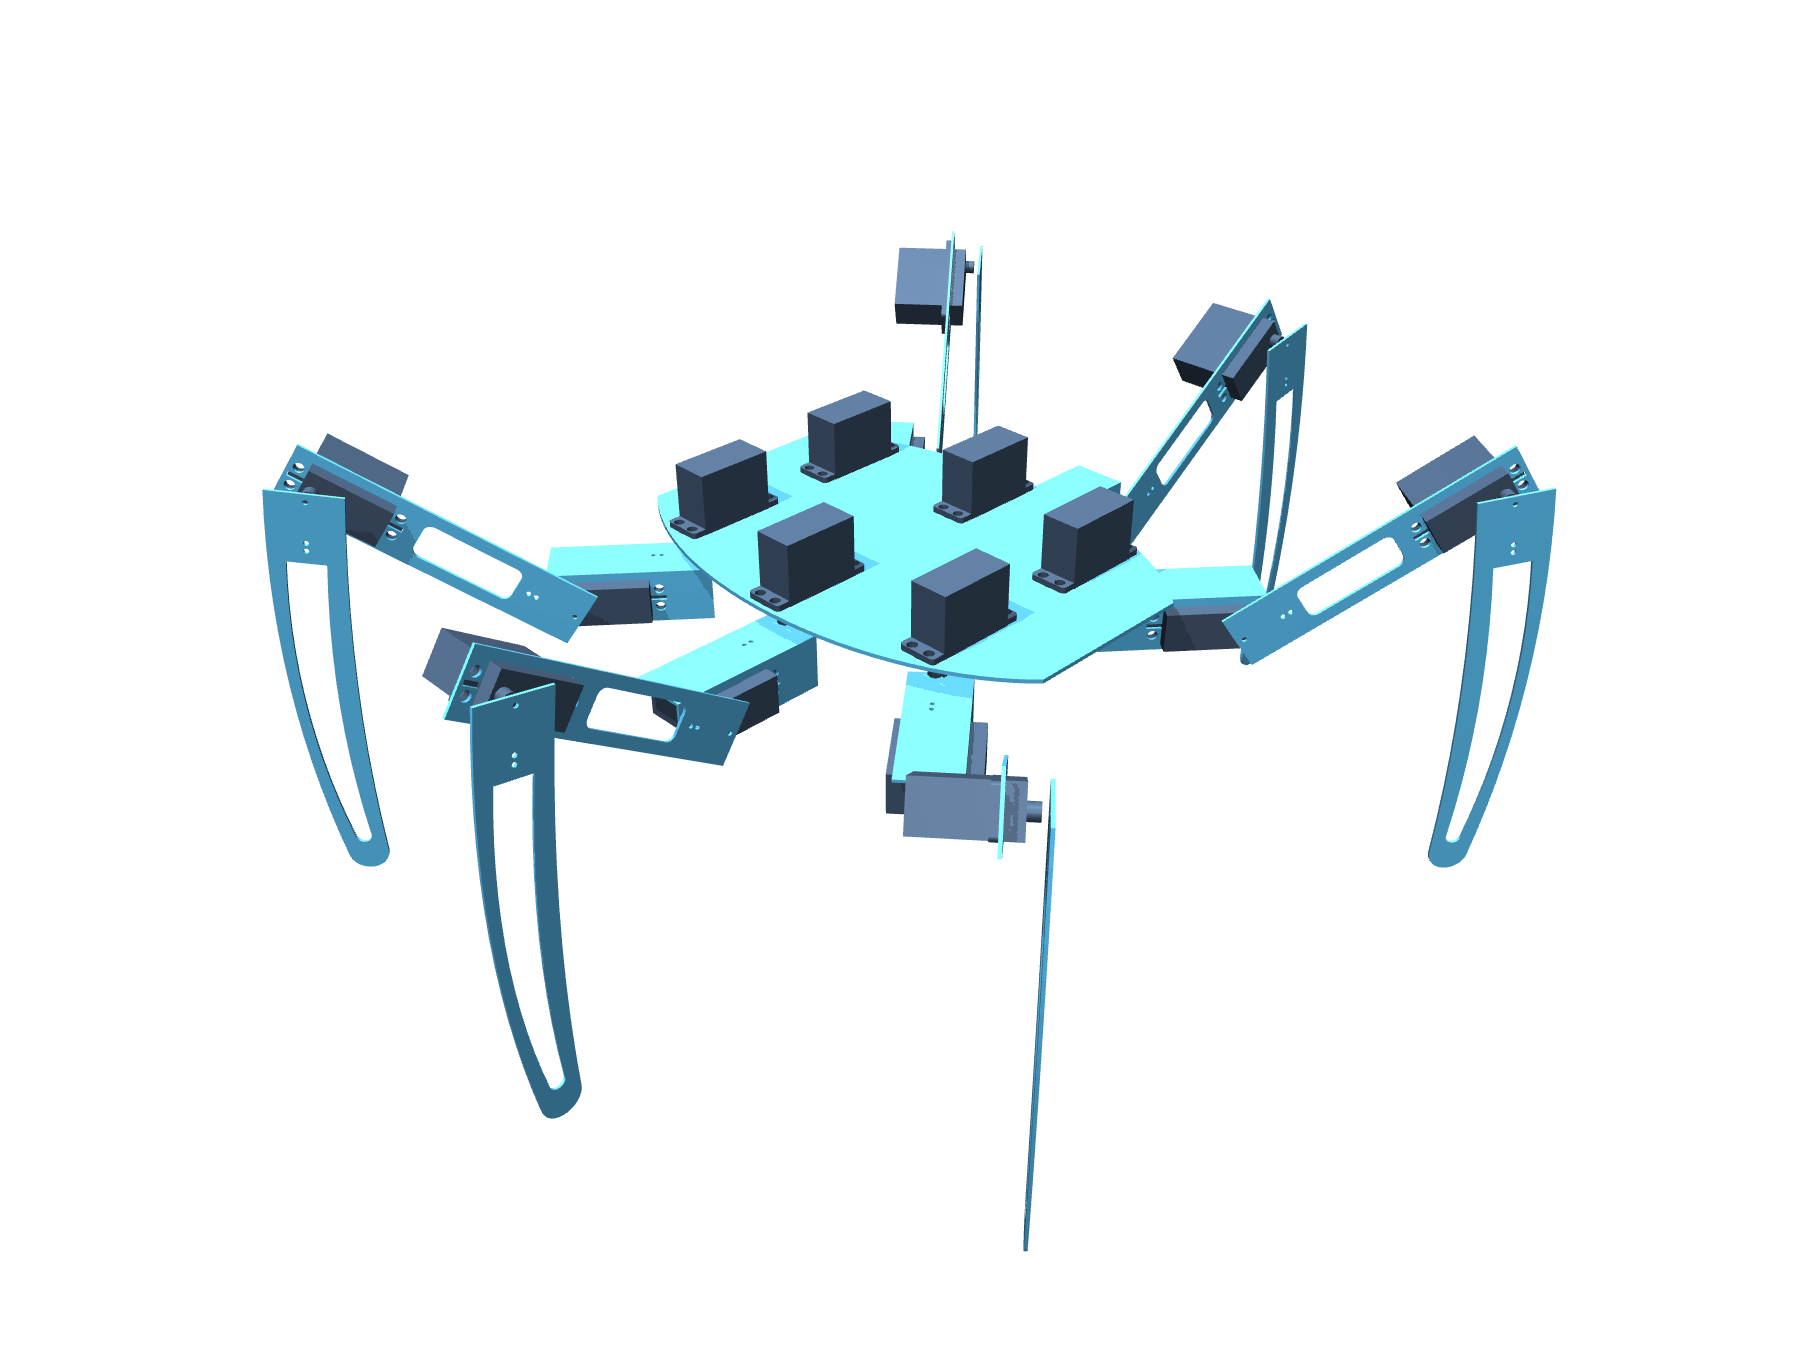
\includegraphics[width=1.65cm,height=.98cm,trim=200 60 200 200,clip,keepaspectratio]{hexapod_model.png}};
\node[small] at (.75,.96) {MuJoCo hexapod};
\node[tiny,text=grey] at (.75,.62) {next body state};

\draw[arrow short,draw=blue] (obs.south) -- (enc.north);
\draw[arrow short,draw=blue] (enc.south) -- (core.north);
\draw[arrow short,draw=orange] (core.south) -- (dec.north);
\draw[arrow short,draw=blue] (dec.south) -- (body.north);

% Explicit closed loop, routed outside all nodes.
\draw[residual,draw=purple] (body.east) -- (3.78,.85);
\draw[draw=purple,densely dashed,line width=.8pt] (3.78,.85) -- (3.78,6.08);
\draw[residual,draw=purple] (3.78,6.08) -- (obs.east);
% Compact plan panel: distinct from the completed fixed-interface results.
\draw[draw=orange!65,fill=orangebg,rounded corners=3pt,dashed,line width=.75pt]
  (-3.4,-1.39) rectangle (3.4,-.12);
\node[font=\sffamily\bfseries\fontsize{7.4}{8.6}\selectfont,text=orange]
  at (0,-.38) {Planned tests (outcomes unverified)};
\node[small,anchor=west] at (-3.12,-.70)
  {1. train on reached states + teacher actions};
\node[small,anchor=west] at (-3.12,-.99)
  {2. score stepping, falls, and targets reached};
\node[small,anchor=west] at (-3.12,-1.28)
  {3. compare measured, shuffled, and rewired graphs};

% Minimal legend: learned vs frozen vs feedback.
\draw[blue,line width=1.5pt] (-3.38,-1.63) -- (-3.05,-1.63);
\node[tiny,anchor=west] at (-2.93,-1.63) {learned};
\draw[orange,line width=1.5pt] (-.95,-1.63) -- (-.62,-1.63);
\node[tiny,anchor=west] at (-.50,-1.63) {frozen};
\draw[purple,densely dashed,line width=1.0pt] (1.30,-1.63) -- (1.63,-1.63);
\node[tiny,anchor=west] at (1.75,-1.63) {body feedback};

\end{tikzpicture}
\end{document}
